%=====================================================================
%  PROJECT REPORT
%  A Digital-Twin and Physical-Watermarking Testbed for Multi-Layer
%  Intrusion Detection in SCADA Systems
%
%  Single-column project report. Compiles on Overleaf with pdfLaTeX.
%  Figures are in ./figures/ (4 screenshots). The architecture diagram,
%  the data-flow flowchart and the results chart are drawn with TikZ/pgfplots.
%=====================================================================
\documentclass[11pt,a4paper]{article}

\usepackage[margin=1in]{geometry}
\usepackage{amsmath,amssymb}
\usepackage{graphicx}
\usepackage{booktabs}
\usepackage{array}
\usepackage{xcolor}
\usepackage{tikz}
\usepackage{pgfplots}
\usepackage{caption}
\usepackage{enumitem}
\usepackage[hidelinks]{hyperref}
\usetikzlibrary{shapes.geometric,arrows.meta,positioning,calc,fit,backgrounds}
\pgfplotsset{compat=1.17}
\captionsetup{font=small,labelfont=bf}
\setlist{nosep,leftmargin=1.5em}

\definecolor{acc}{HTML}{E0572F}
\definecolor{lnet}{HTML}{3B82C4}
\definecolor{lproc}{HTML}{8B5CF6}
\definecolor{ltwin}{HTML}{1F9D5A}
\definecolor{lwm}{HTML}{C79400}
\definecolor{slate}{HTML}{334155}
\definecolor{lightgray}{HTML}{EEF1F5}

\begin{document}

%--------------------------------------------------------------- title
\begin{titlepage}
\centering
\vspace*{2cm}
{\LARGE\bfseries A Digital-Twin and Physical-Watermarking Testbed for Multi-Layer Intrusion Detection in SCADA Systems\par}
\vspace{0.6cm}
{\large Project Report\par}
\vspace{2cm}
{\large\bfseries
S. Saurabh Krishnan \quad Hemant Bhupesh \\[4pt]
Sanjai S \quad Nitesh V. M.\par}
\vspace{0.8cm}
{\large Amrita Vishwa Vidyapeetham, Coimbatore, India\par}
\vfill
{\itshape Educational research simulation --- all devices, telemetry and attacks are synthetic and local.\par}
\vspace{1cm}
\end{titlepage}

\tableofcontents
\newpage

%--------------------------------------------------------------- abstract
\section*{Abstract}
\addcontentsline{toc}{section}{Abstract}
Industrial supervisory control and data acquisition (SCADA) systems are increasingly targeted by attacks that falsify sensor telemetry or inject unauthorised control commands. Conventional network intrusion detection observes only the communication layer and is therefore blind to attacks that manipulate a field device directly. This report presents a fully simulated, reproducible cyber-physical security testbed built around a liquid-metal boiler plant, and uses it to evaluate a defence that combines four complementary detection layers---network, process, an independent digital twin, and physical watermarking---fused by a correlation engine. The digital twin integrates its own physics model with datasheet parameters and a gated measurement-fusion rule, so a falsified reading produces a growing, detectable residual rather than silently corrupting the estimate. A bounded pseudo-random watermark is injected into an actuator command and its effect is checked against the twin-predicted response. Across ten reproducible attack scenarios, a network-only detector misses sensor-falsification attacks entirely ($F_1 = 0.00$) while the full multi-layer stack detects them within $0.2$\,s ($F_1 = 0.94$); conversely, command-path attacks are caught by the network layer, demonstrating that the layers are genuinely complementary. The platform runs live in a browser with a 10\,Hz simulation, an operator HMI and an automated response engine, and is released with 56 automated tests.

\medskip
\noindent\textbf{Keywords:} SCADA security, digital twin, intrusion detection, physical watermarking, cyber-physical systems, false data injection.

%--------------------------------------------------------------- introduction
\section{Introduction}
Modern industrial plants are controlled by SCADA systems in which programmable logic controllers (PLCs) drive actuators and read sensors, while a supervisory server polls those controllers over industrial protocols such as Modbus TCP, OPC~UA and MQTT. The convergence of operational technology (OT) with commodity networking has widened the attack surface: incidents such as Stuxnet~\cite{stuxnet}, the 2015--2016 attacks on the Ukrainian power grid~\cite{ukraine}, and the TRITON/TRISIS safety-system malware show that adversaries can falsify measurements, replay or inject control commands, and tamper with field devices.

A defender who watches only network traffic faces a fundamental blind spot. An attacker who compromises a field device, or who sits between a sensor and its controller, can present a plausible but false value to the operator while the physical process diverges. The network sees a well-formed packet; nothing in the communication layer is anomalous. Detecting such attacks requires reasoning about the physics of the process, not only its packets~\cite{cardenas,urbina}.

\subsection{Objective and scope}
The objective of this project is to build a self-contained, reproducible testbed in which such cyber-physical attacks can be studied, and to use it to demonstrate quantitatively that a multi-layer defence is required. Specifically, the project delivers:
\begin{enumerate}
\item a simulated liquid-metal boiler plant with 37 sensors, 17 actuators, five PLCs/RTU and a Purdue-zoned control network, running live at 10\,Hz with an operator HMI;
\item an \emph{independent} digital twin that fuses measurements through a gated correction, so that falsified telemetry is exposed rather than absorbed;
\item a four-layer intrusion detection system (network, process, twin, watermark) with a correlation engine;
\item a functional physical-watermarking engine;
\item an attack laboratory of ten reproducible scenarios with ground-truth labelling, and a quantitative evaluation of detector complementarity.
\end{enumerate}
The platform is an educational and research simulation: the process model is a simplified, plausible abstraction, not a validated engineering or safety model.

%--------------------------------------------------------------- methodology
\section{Methodology}
\subsection{System architecture}
The platform is organised as a layered stack (Fig.~\ref{fig:arch}). A single simulation engine advances the whole system at a fixed timestep ($dt = 0.1$\,s, i.e.\ 10\,Hz) and executes a fixed per-tick sequence (Fig.~\ref{fig:flow}). Four design invariants make the security evaluation meaningful: (i) the attacker can touch only the network and field-device firmware hooks---never the safety system, twin, IDS or watermark engine; (ii) the twin never reads ground-truth state; (iii) the safety system is independent of the network and the response engine; and (iv) ground-truth attack labels reach the evaluator only, never the detectors.

\begin{figure}[t]
\centering
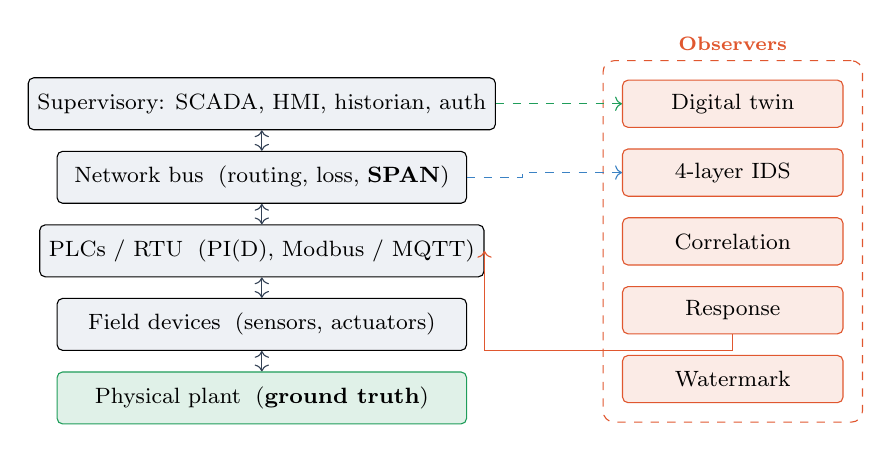
\begin{tikzpicture}[font=\footnotesize,node distance=2.6mm,
  layer/.style={draw,rounded corners=2pt,minimum width=52mm,minimum height=6.6mm,align=center,fill=lightgray},
  obs/.style={draw,rounded corners=2pt,minimum width=28mm,minimum height=6mm,align=center,fill=acc!12,draw=acc}]
\node[layer] (sup) {Supervisory: SCADA, HMI, historian, auth};
\node[layer,below=of sup] (net) {Network bus \;(routing, loss, \textbf{SPAN})};
\node[layer,below=of net] (plc) {PLCs / RTU \;(PI(D), Modbus / MQTT)};
\node[layer,below=of plc] (fld) {Field devices \;(sensors, actuators)};
\node[layer,below=of fld,fill=ltwin!14,draw=ltwin] (phy) {Physical plant \;(\textbf{ground truth})};
\draw[<->,slate] (sup)--(net); \draw[<->,slate] (net)--(plc);
\draw[<->,slate] (plc)--(fld); \draw[<->,slate] (fld)--(phy);
\node[obs,right=16mm of sup] (twin) {Digital twin};
\node[obs,below=of twin] (ids) {4-layer IDS};
\node[obs,below=of ids] (corr) {Correlation};
\node[obs,below=of corr] (resp) {Response};
\node[obs,below=of resp] (wmk) {Watermark};
\begin{scope}[on background layer]
\node[draw=acc,dashed,rounded corners,fit=(twin)(wmk),inner sep=2.4mm,label=above:{\scriptsize\color{acc}\textbf{Observers}}] {};
\end{scope}
\draw[->,lnet,dashed] (net.east) -- ++(7mm,0) |- (ids.west);
\draw[->,ltwin,dashed] (sup.east) -- ++(11mm,0) |- (twin.west);
\draw[->,acc] (resp.south) -- ++(0,-2mm) -| (plc.east);
\end{tikzpicture}
\caption{Layered architecture. The attacker may touch only the network and field devices; the observers tap the stack, and the response engine acts on simulated components.}
\label{fig:arch}
\end{figure}

\begin{figure}[t]
\centering
\begin{tikzpicture}[font=\scriptsize,node distance=3.2mm,
  step/.style={draw,rounded corners=3pt,minimum width=72mm,minimum height=5.6mm,align=center,fill=lightgray},
  hot/.style={step,fill=acc!15,draw=acc},
  grn/.style={step,fill=ltwin!14,draw=ltwin},
  arr/.style={-{Stealth[length=2mm]},slate,thick}]
\node[hot] (s1) {1.\ Attack lab applies manipulations};
\node[grn,below=of s1] (s2) {2.\ Physical plant integrates (ground truth)};
\node[grn,below=of s2] (s3) {3.\ Hard-wired safety (SIS) may trip final elements};
\node[step,below=of s3] (s4) {4.\ Field I/O: sensors sample, PLCs scan};
\node[step,below=of s4] (s5) {5.\ Network bus delivers messages (SPAN mirror)};
\node[step,below=of s5] (s6) {6.\ SCADA polling, historian \& twin feeds};
\node[step,below=of s6] (s7) {7.\ Digital twin + watermark update};
\node[step,below=of s7] (s8) {8.\ IDS (4 layers) $\rightarrow$ correlation};
\node[hot,below=of s8] (s9) {9.\ Response engine \;$\rightarrow$\; snapshot emitted};
\draw[arr] (s1)--(s2); \draw[arr] (s2)--(s3); \draw[arr] (s3)--(s4);
\draw[arr] (s4)--(s5); \draw[arr] (s5)--(s6); \draw[arr] (s6)--(s7);
\draw[arr] (s7)--(s8); \draw[arr] (s8)--(s9);
\end{tikzpicture}
\caption{Per-tick data-flow of the simulation engine (10\,Hz). Green steps read the true plant state; the attacker (step~1) and the SPAN-fed IDS (steps~5--8) never see it.}
\label{fig:flow}
\end{figure}

\subsection{Process and plant model}
The primary plant is a lumped-parameter liquid-metal boiler with an intermediate heat exchanger (IHX), a secondary water loop and a turbine-generator. The bulk vessel temperature evolves as a heat balance:
\begin{equation}
C_b\,\frac{dT_b}{dt}=Q_{\text{heater}}-\dot{m}\,c_p\,(T_b-T_{\text{cl}})-UA_{\text{loss}}\,(T_b-T_{\text{amb}})
\end{equation}
The IHX uses a counter-flow effectiveness--NTU relation, and the secondary loop and generator follow first-order dynamics. Four auxiliary subsystems reuse the same abstractions: an induction motor, a water-treatment plant, a batch chemical-mixing reactor, and a pipeline/tank farm. Each sensor turns the true value into a measurement via noise, quantisation and range clamping; each actuator applies a rate limit and lag. A separate Safety Instrumented System (SIS) reads the plant through its own instruments, is not on the network, and trips final elements \emph{after} any firmware tampering.

\subsection{Network and protocols}
The network is a Purdue-zoned graph (supervisory L2, an industrial firewall, control L1, and a cellular link to a remote RTU). Modbus TCP is encoded and decoded as spec-conformant application data units (MBAP header plus PDU)~\cite{modbus}; OPC~UA and MQTT are modelled at the application level. A discrete-event bus carries every message with latency, jitter and loss, and mirrors supervisory traffic to the IDS through a SPAN port.

\subsection{Independent digital twin}
The twin integrates its own copy of the primary-loop physics with a fourth-order Runge--Kutta scheme and datasheet parameters that differ from the plant by a few percent. Its inputs are the issued commands (plus the trusted watermark offset) and a few measured drivers; it never reads ground-truth state. Each tick it forms a one-step-ahead prediction $\hat{y}_k$ and applies a gated correction. The residual and normalised innovation are:
\begin{equation}
r_k=y_k-\hat{y}_k,\qquad z_k=\frac{r_k-b_k}{\sigma_k}
\end{equation}
A measurement updates the state only if $|z_k|<5$; readings outside the gate are rejected, so a falsified sensor cannot silently drag the twin along. Residuals feed a two-sided CUSUM statistic and a sudden-error counter.

\subsection{Multi-layer intrusion detection}
Four independent detectors are used. The \textbf{network} layer (SPAN mirror only) flags rogue devices, spoofing, unexpected flows, floods, invalid sequences, replays and unauthorised writes. The \textbf{process} layer flags limit violations, frozen signals, implausible rate-of-change, setpoint deviation, pump-flow inconsistency and energy-balance violations. The \textbf{digital-twin} layer flags persistent and sudden residuals. The \textbf{watermark} layer contributes its decision. A correlation engine deduplicates findings into incidents and combines per-layer confidence as
\begin{equation}
C=1-\prod_{i}\bigl(1-c_i\bigr),
\end{equation}
raising severity per corroborating layer and classifying the incident with transparent rules.

\subsection{Physical watermarking}
A reproducible, bounded pseudo-random binary sequence (PRBS) is injected into an actuator command inside the PLC's secured function block; the exported register still reports the operator's base value. Two shadow copies of the twin's hydraulics compute the \emph{expected} response; high-pass-filtered telemetry gives the \emph{observed} response. Per channel the detector computes the correlation $\rho$, the response gain and an SNR, returning \textit{consistent}, \textit{suspicious}, or \textit{inconclusive}. Injection self-suspends on a safety trip, near saturation, close to a process limit, or when measurement quality is poor.

\subsection{Attack laboratory and evaluation}
Ten reproducible scenarios exercise the detectors (false data injection, frozen readings, actuator manipulation, unauthorised setpoint, command replay, denial of service, insider writes, twin tampering, watermark interference, coordinated attack). Each records its seed, produces real changes, exposes a ground-truth label, and supports stop/recover. Experiments run a deterministic engine (seed 1337) through baseline, attack and recovery phases; the \emph{same} recorded trace is scored under four detector configurations so the comparison is apples-to-apples. Each 2\,s window is positive if the attack was active for at least half of it, and detected if a non-info finding mapped to the attacked zone. We report precision, recall, $F_1$ and detection latency.

%--------------------------------------------------------------- implementation
\section{Implementation}
\subsection{Technology stack}
The backend is implemented in Python with FastAPI and Uvicorn; the physical model uses NumPy/SciPy. The frontend is a React~+~TypeScript single-page application built with Vite and styled with Tailwind CSS, using Recharts for time-series and React~Flow for the network graph. Live state is pushed to the browser over a WebSocket at up to 10\,Hz, a REST API exposes control and query endpoints, and SQLite persists alerts, incidents, events, responses and experiment results. The whole platform launches with a single command and is deterministic for a given master seed.

\subsection{Modules and scale}
The simulation comprises 37 sensors, 17 actuators, five controllers (four Modbus PLCs and one MQTT RTU) and a 72-node Purdue-zoned network. The backend is organised into clearly separated subsystems: \texttt{simulation} (plant, devices, PLCs, safety), \texttt{network} (topology, protocols, discrete-event bus), \texttt{digital\_twin}, \texttt{ids} (four detectors + correlation), \texttt{watermarking}, \texttt{attacks}, \texttt{response}, \texttt{experiments} and \texttt{storage}. Correctness is guarded by 56 automated tests covering the process model, safety independence, twin independence, residuals, watermark generation and evaluation, each IDS layer, correlation, responses, API validation, WebSocket telemetry, persistence and the experiment metrics.

\subsection{Operator HMI}
The HMI presents eight pages. The Plant Overview (Fig.~\ref{fig:plant}) shows an animated P\&ID with live telemetry, alarm states and the independent safety panel. The Network Topology page (Fig.~\ref{fig:net}) renders the interactive Purdue graph with the live SPAN-mirrored traffic. The Digital Twin page (Fig.~\ref{fig:twin}) plots predicted vs.\ observed values and residuals. The Security Center (Fig.~\ref{fig:sec}) shows the alert feed, correlated incidents and the response timeline. Further pages cover the device inventory, the watermarking signal/decision, the attack laboratory and the experiment analytics.

\begin{figure}[t]
\centering
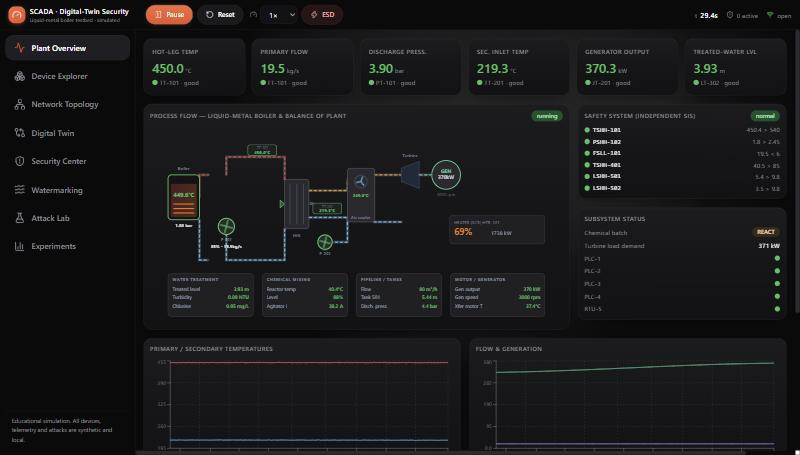
\includegraphics[width=0.86\textwidth]{figures/plant_overview.jpg}
\caption{Plant Overview: the animated P\&ID of the liquid-metal boiler, balance-of-plant tiles, independent safety panel and live trend charts.}
\label{fig:plant}
\end{figure}

\begin{figure}[t]
\centering
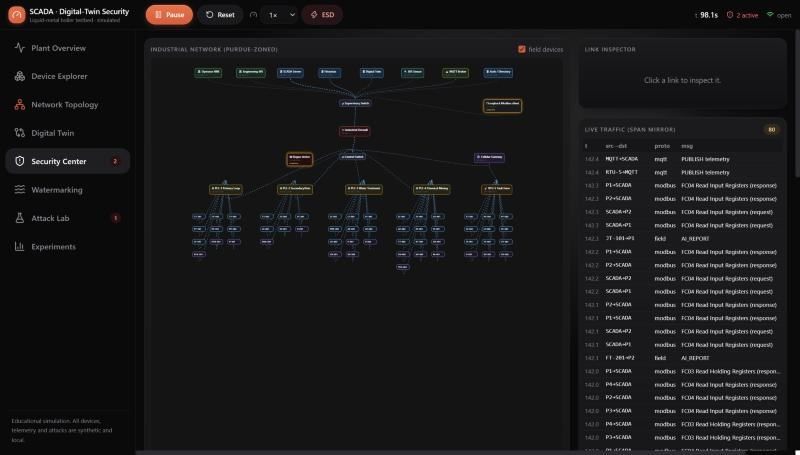
\includegraphics[width=0.86\textwidth]{figures/network_topology.jpg}
\caption{Network Topology: the Purdue-zoned network and the live SPAN-mirrored Modbus/MQTT traffic fed to the IDS.}
\label{fig:net}
\end{figure}

%--------------------------------------------------------------- results
\section{Results}
Table~\ref{tab:results} reports the detection $F_1$ of each configuration across the scenario suite; Fig.~\ref{fig:bars} isolates the two telemetry-falsification attacks.

\begin{table}[t]
\centering
\caption{Detection $F_1$ by detector configuration (seed 1337, 2\,s windows). ``miss'' = no detection.}
\label{tab:results}
\renewcommand{\arraystretch}{1.25}
\begin{tabular}{@{}lccccc@{}}
\toprule
\textbf{Scenario} & \textbf{Net only} & \textbf{Net+Proc} & \textbf{+Twin} & \textbf{Full+WM} & \textbf{Latency}\\
\midrule
A. Normal operation      & --   & --   & --   & --   & --\\
B. False data injection   & \textcolor{red}{miss} & 0.94 & 0.94 & \textbf{0.94} & 0.2\,s\\
C. Watermark interference & \textcolor{red}{miss} & \textcolor{red}{miss} & 0.71 & \textbf{0.96} & 1.1\,s\\
D. Unauthorised setpoint  & 0.91 & 0.91 & 0.91 & \textbf{0.91} & 0.0\,s\\
E. Command replay         & 0.93 & 0.93 & 0.93 & \textbf{0.93} & 0.5\,s\\
F. Coordinated            & 0.91 & 0.91 & 0.91 & \textbf{0.91} & 0.5\,s\\
\bottomrule
\end{tabular}
\end{table}

\begin{figure}[t]
\centering
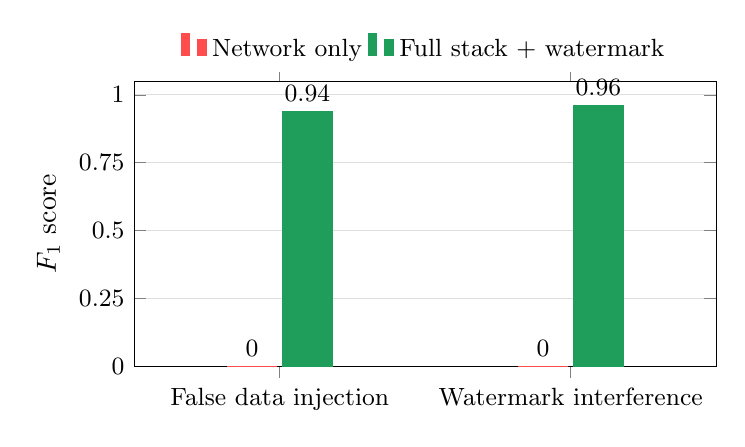
\begin{tikzpicture}
\begin{axis}[
  width=0.74\textwidth, height=52mm,
  ybar, bar width=18pt, enlarge x limits=0.5,
  ymin=0, ymax=1.05, ytick={0,0.25,0.5,0.75,1.0},
  ylabel={$F_1$ score},
  symbolic x coords={False data injection, Watermark interference},
  xtick=data, tick label style={font=\small},
  legend style={font=\small,at={(0.5,1.03)},anchor=south,legend columns=2,draw=none},
  nodes near coords, every node near coord/.append style={font=\small,/pgf/number format/fixed,/pgf/number format/precision=2},
  ymajorgrids, grid style={gray!25},
]
\addplot[fill=red!70,draw=red!70] coordinates {(False data injection,0.0) (Watermark interference,0.0)};
\addplot[fill=ltwin,draw=ltwin] coordinates {(False data injection,0.94) (Watermark interference,0.96)};
\legend{Network only, Full stack + watermark}
\end{axis}
\end{tikzpicture}
\caption{On telemetry-falsification attacks a network-only IDS scores $F_1=0$, while the full multi-layer stack reaches $0.94$--$0.96$.}
\label{fig:bars}
\end{figure}

The results support four observations. (1)~\emph{No false positives in normal operation}: configuration~A raises no sustained alerts. (2)~\emph{Network-only is blind to telemetry falsification}: scenarios~B and~C produce no network-layer evidence and are missed by a packet-only detector; the process and twin layers recover~B within $0.2$\,s. (3)~\emph{The watermark earns its place on~C}: the process layer alone sees nothing, the twin partially catches the slow drift ($F_1=0.71$), and the physical watermark raises detection to $0.96$. (4)~\emph{Command-path attacks are caught on the network}: unauthorised writes~(D), replay~(E) and the coordinated attack~(F) leave direct network evidence and are detected even by network-only.

\begin{figure}[t]
\centering
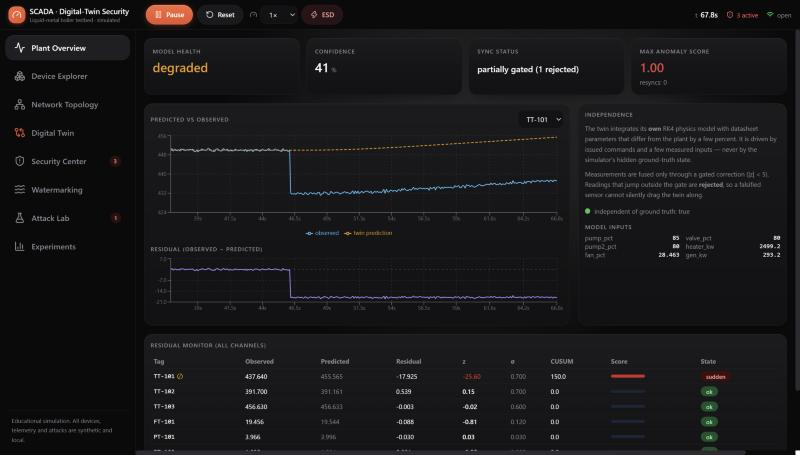
\includegraphics[width=0.86\textwidth]{figures/twin_divergence.jpg}
\caption{Twin view during a false-data injection: the observed value (blue) is pulled to the falsified reading while the twin prediction (orange) tracks the real temperature; the residual reaches $z=-25.6$.}
\label{fig:twin}
\end{figure}

\begin{figure}[t]
\centering
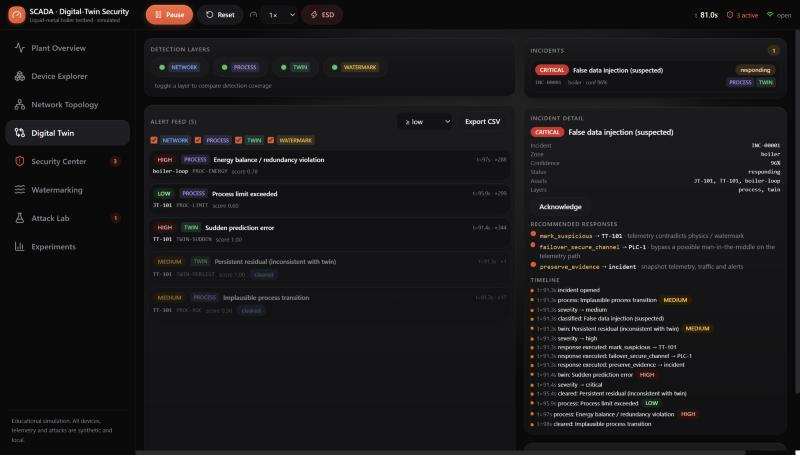
\includegraphics[width=0.86\textwidth]{figures/security_center.jpg}
\caption{Security Center during a false-data injection: the alert feed, the correlated critical incident at 96\% confidence, and the automatically executed responses.}
\label{fig:sec}
\end{figure}

In a live run of scenario~B, the real hot-leg temperature rose to $459.8\,^{\circ}$C while SCADA displayed the falsified $442.3\,^{\circ}$C (Fig.~\ref{fig:twin}); the twin residual reached $z=-24.9$ with a saturated CUSUM, and the correlation engine raised a critical ``False data injection'' incident at 0.96 confidence, after which the automatic response quarantined the source, restored the setpoint and preserved evidence (Fig.~\ref{fig:sec}). The plant returned to a healthy, synchronised state once the scenario was stopped. The few false positives in B--F are post-attack recovery transients.

%--------------------------------------------------------------- conclusion
\section{Conclusion and Future Work}
We presented a self-contained, reproducible cyber-physical security testbed that couples a simulated SCADA plant with an independent digital twin, a four-layer intrusion detection system, a physical-watermarking engine, an attack laboratory and an automated response engine, all running live at 10\,Hz with an operator HMI. We showed quantitatively that the detection layers are complementary: network-only detection is blind to telemetry falsification while the multi-layer stack detects it within fractions of a second, and the physical watermark adds detection value precisely where passive layers fail.

The main limitation is that the process model is a simplified, hypothetical abstraction, not a validated engineering model, and that OPC~UA and MQTT are emulated at the application level. Because the twin shares a model family with the plant, a sufficiently slow in-gate ramp can still bias it. Future work includes characterising the stealthy in-gate ramp boundary, adding learning-based detectors alongside the transparent rules, broadening the stochastic evaluation across many seeds, and binding real protocol libraries over an isolated loopback network.

%--------------------------------------------------------------- contributions
\section*{Author Contributions}
\addcontentsline{toc}{section}{Author Contributions}
\begin{itemize}
\item \textbf{S. Saurabh Krishnan} --- Digital twin (independent RK4 model, gated correction, residual/CUSUM analysis, model-confidence and synchronisation) and the reproducible experiment/metrics framework and 56-test suite.
\item \textbf{Hemant Bhupesh} --- Plant and network simulation: the boiler and auxiliary subsystems, device abstractions, PLC/RTU control programs, the hard-wired safety system, and the Purdue-zoned network, discrete-event bus and protocol layer.
\item \textbf{Sanjai S} --- Multi-layer intrusion detection (network, process, twin and watermark detectors and the energy-balance checks), the correlation engine, the ten attack scenarios, and the automated defensive-response engine.
\item \textbf{Nitesh V. M.} --- Physical watermarking (PRBS signal, shadow-model response and the correlation/gain/SNR detector), the React/TypeScript operator HMI, the FastAPI REST/WebSocket backend and SQLite persistence, and the report and documentation.
\end{itemize}

%--------------------------------------------------------------- references
\begin{thebibliography}{00}
\bibitem{stuxnet} N. Falliere, L. O. Murchu, and E. Chien, ``W32.Stuxnet Dossier,'' Symantec Security Response, 2011.
\bibitem{mo2009} Y. Mo and B. Sinopoli, ``Secure control against replay attacks,'' in \textit{Proc. 47th Allerton Conf.}, 2009, pp. 911--918.
\bibitem{mo2015} Y. Mo, S. Weerakkody, and B. Sinopoli, ``Physical authentication of control systems,'' \textit{IEEE Control Syst. Mag.}, vol. 35, no. 1, pp. 93--109, 2015.
\bibitem{cardenas} A. A. C\'ardenas \textit{et al.}, ``Attacks against process control systems: Risk assessment, detection, and response,'' in \textit{Proc. ACM ASIACCS}, 2011, pp. 355--366.
\bibitem{urbina} D. Urbina \textit{et al.}, ``Limiting the impact of stealthy attacks on industrial control systems,'' in \textit{Proc. ACM CCS}, 2016, pp. 1092--1105.
\bibitem{modbus} Modbus Organization, ``Modbus Application Protocol Specification V1.1b3,'' 2012.
\bibitem{ukraine} R. M. Lee, M. J. Assante, and T. Conway, ``Analysis of the cyber attack on the Ukrainian power grid,'' E-ISAC/SANS, 2016.
\end{thebibliography}

\end{document}
